\section{SOTA of object detection}
\subsection{Introduction to Object Detection}
\href{https://www.mathworks.com/discovery/object-detection.html#:~:text=Object%20detection%20is%20a%20computer,learning%20to%20produce%20meaningful%20results.}{Object detection} Object detection is a vital computer vision technique which is employed to identify instances of objects within images or videos. This technique is commonly implemented through the use of machine learning or deep learning algorithms, which are responsible for producing robust and accurate results. While humans are able to quickly recognize and locate objects of interest within visual data, the ultimate goal of object detection is to replicate this cognitive ability using computational methods. By detecting and localizing objects within visual data, object detection has become a crucial tool for various computer vision applications, including robotics, autonomous vehicles, and surveillance systems. \cite{zhao2019object}, \cite{ansari2020building}
\subsubsection{Why Object Detection}
Identifying and localizing objects within an image or video is called object detection and is a fundamental task in computer vision. It plays a pivotal role in various real-world applications, contributing to advancements in technology and enhancing our daily lives. The importance of object detection lies in its ability to enable machines to interpret and understand visual information, allowing them to make informed decisions and interact intelligently with the environment.\cite{pathak2018application}, 
\begin{enumerate}
    \item \textbf{Automation and Efficiency:} Object detection is a cornerstone in developing automated systems, empowering machines to perceive and respond to their surroundings. This is particularly crucial in industries such as manufacturing, where the automation of tasks, such as quality control and inventory management, leads to increased efficiency and reduced operational costs.
    \item \textbf{Enhanced Security and Surveillance:}  In the realm of security and surveillance, object detection is instrumental in identifying potential threats or anomalies. Surveillance cameras equipped with object detection algorithms can automatically detect and alert authorities to suspicious activities, enhancing public safety in crowded spaces, transportation hubs, and critical infrastructure.
    \item \textbf{Autonomous Vehicles:} The advent of autonomous vehicles relies heavily on object detection to interpret the dynamic environment. Cars equipped with object detection systems can identify pedestrians, vehicles, and obstacles, enabling safer navigation and reducing the likelihood of accidents.
    \item \textbf{Medical Imaging and Diagnosis:}  In the field of healthcare, object detection plays a vital role in medical imaging. It aids in detecting and localizing abnormalities in radiological images, facilitating early diagnosis and improving patient outcomes.
    \item \textbf{Retail and Customer Experience:} Object detection is utilized in retail for tasks such as inventory management, shelf monitoring, and cashierless checkout systems. These applications streamline operations and enhance customer experience by reducing waiting times and optimizing stock levels.
\end{enumerate}

\textbf{Real-world Scenarios:}\\
\begin{enumerate}
    \item \textbf{Smart Cities:} Object detection is integral to developing smart cities. It can be used in urban environments for traffic management, waste management, and monitoring public spaces, contributing to more efficient and sustainable urban living.
    \item \textbf{Search and Rescue Operations:} In disaster-stricken areas, object detection aids in search and rescue operations by identifying and locating individuals needing assistance. Drones equipped with object detection capabilities can quickly cover large areas, improving rescue efforts' efficiency.
    \item \textbf{Environmental Monitoring: } Object detection is applied in environmental science for monitoring wildlife, tracking deforestation, and studying biodiversity. It enables researchers to gather crucial data for conservation and ecological studies.
    \item \textbf{Augmented Reality:} Object detection is a key component in augmented reality applications, where virtual elements are seamlessly integrated with the real world. This technology enhances user experiences in gaming, education, and various interactive scenarios.
\end{enumerate} \cite{ansari2020building}, \cite{pathak2018application}

\subsection{Object detection stage}
Object detection can be classified into two stages according to the detection process steps:
\begin{itemize}
    \item \textbf{One-stage detector}  is a simple regression problem that takes input and learns probability classes and bounding box coordinates. YOLO, YOLO v2, SSD, RetinaNet, etc., fall under one-phase detectors. Object detection is an advanced form of imaging classification where a neural network predicts objects in an image and draws attention to them in the form of bounding boxes. \cite{oneStage}
    \item \textbf{Two-stage detector} A two-stage detector completes detection in two steps. In the first step, regional design networks are used to create areas of interest with a high probability of being objects. In the second step, object detection is performed, which includes the final classification and regression of the bounding box of the detected objects. RCNN, Fast RCNN, SPPNET, Faster RCNN, etc., are some of the two-stage detectors. \cite{du2020overview}
\end{itemize}

\begin{figure}[H]
    \centering
    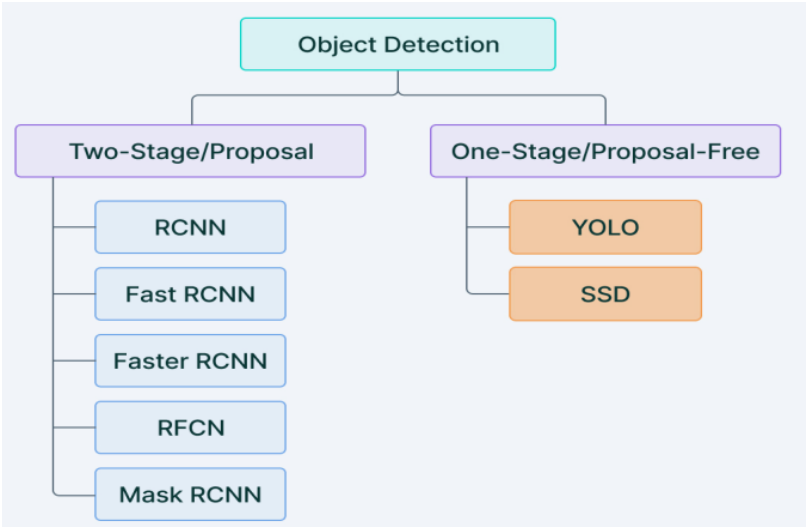
\includegraphics[width=0.7\textwidth]{ObjectDetection_Stage.PNG}
    \caption{Stage  or classification of Object Detection}
    \label{fig: Stage of Object Detection}
\end{figure}

\subsection{Two-Stage/Proposal: }
  Two-stage object detection algorithms typically have two steps: region proposal and object classification or refinement. One popular framework is the region-based Convolutional Neural Network (R-CNN) and its variants.\cite{du2020overview}, \cite{ansari2020building}
\subsubsection{Region-Based Convolutional Neural Network: } \underline{\textcolor{blue}{\href{https://arxiv.org/pdf/1311.2524.pdf}{R-CNN}}}
A Region-Based Convolutional Neural Network (R-CNN) is a type of neural network specifically designed to detect objects in images. R-CNN uses region proposals generated by a selective search (SS) approach to pre-compute the priors. Since the features between these regions are not shared, we need to extract features individually for each region of interest (RoI) generated using an SS approach. Unlike other neural networks, R-CNNs are designed not only to classify objects but also to locate and delineate their boundaries within the image.
The R-CNN architecture was first proposed in 2014 by Ross Girshick, Jeff Donahue, Trevor Darrell, and Jitendra Malik in their paper titled "Rich Feature Hierarchies for Accurate Object Detection and Semantic Segmentation." Since then, the architecture has undergone several iterations, including Fast R-CNN, Faster R-CNN, and Mask R-CNN.
        
    \begin{figure}[H]
         \centering
         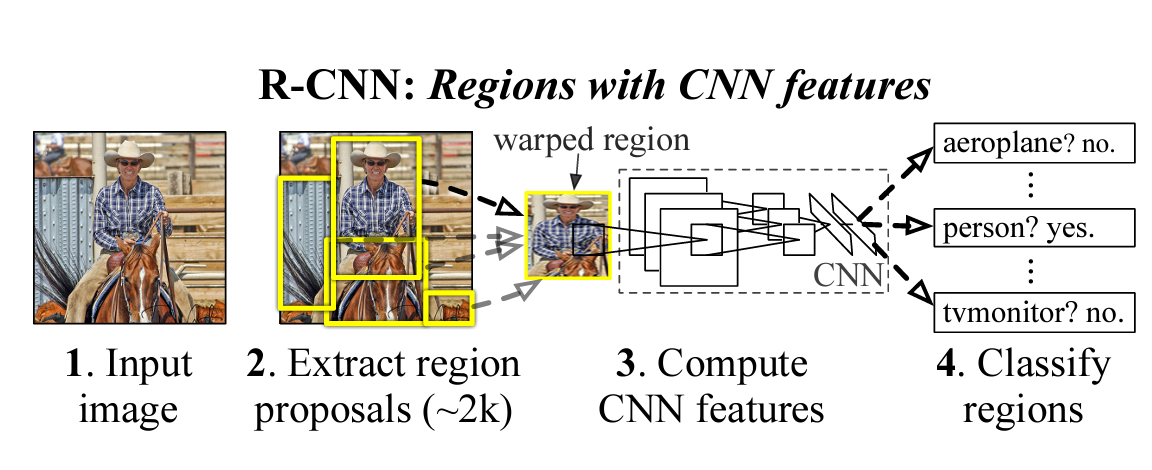
\includegraphics[width=0.6\textwidth]{R_CNN.PNG}
         \caption{R-CNN Model(Source:\cite{girshick2014rich})}
            \label{fig: R-CNN Model}
    \end{figure}
\textbf{R-CNN comprises of the following three modules:}\\
        \begin{enumerate}
            \item \textbf{Region proposal: } The R-CNN algorithm starts by identifying regions in an image that may contain objects. These regions are known as region proposals. They are referred to as proposals because they may or may not contain objects, and the goal of the learning function is to remove areas that do not contain objects. Region proposals are bounding boxes around the objects.
            \item \textbf{Feature extraction:} To identify objects in an image, the first step is to crop out the region proposals and resize them. These resized images are then sent through a standard CNN for feature extraction. The original research paper employed AlexNet for this purpose. The CNN extracts 4,096-dimensional feature vectors from each region.
            \item  \textbf{Classifier: } The extracted features are classified by using the standard classification algorithms, such as the linear SVM model 
        \end{enumerate}
R-CNN was the first successful deep learning–based object detection system, but it suffered a serious issue concerning performance. Its time performance problem is because of the following:
    \begin{itemize}
         \item For feature extraction, each region proposal undergoes approximately 2,000 passes per image in the CNN.
        \item Three models are trained: CNN for feature extraction, classifier for image class prediction, and regression for bounding box refinement. Training is compute-intensive, increasing computation time.
        \item Due to the large number of regions, CNN predictions are slow for each proposal.
    \end{itemize}
        
\subsubsection{Fast R-CNN:} In 2015, Ross Girshick from Microsoft proposed a single model called "Fast R-CNN" to overcome the limitations of R-CNNs. This model learns and outputs region proposals and classifications directly, resulting in higher mAP on PASCAL compared to R-CNN.\cite{girshick2015fast}  

Fast R-CNN trains a deep VGG-16 network that is significantly faster than R-CNN (9x faster during training and 213x faster at test time). The model achieves this speed by evaluating the network and extracting features for the entire image once, instead of extracting features from each region of interest (RoI) as in R-CNN. To extract features from RoIs, Fast R-CNN uses the concept of RoI pooling, which is a special case of pyramid pooling used in SPPNet. 

RoI pooling provides a feature vector of the desired length that is then used for classification and localization. This method is more efficient than R-CNN because the computations for overlapping regions are shared. Overall, Fast R-CNN significantly improves the speed and performance of object detection models.
        

\textbf{Building blocks of Fast R-CNN:}
    \begin{enumerate}
        \item Region proposal network
        \item Feature extraction using CNN
        \item RoI pooling layer: This is where the real magic of Fast R-CNN happens
        \item Classification and Localization
    \end{enumerate}
        
    \begin{figure}[H]
        \centering
        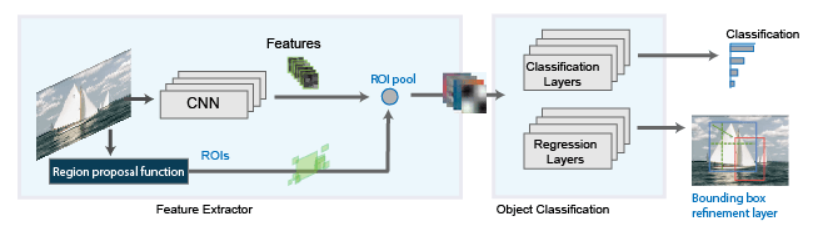
\includegraphics[width=1\textwidth]{Fast_RCNN_ARch.PNG}
        \caption{Architectural Design of Fast R-CNN \cite{girshick2014rich}}
        \label{fig: Fast R-CNN}
    \end{figure}
        
The region proposal network and feature extraction modules work similarly to the ones used in R-CNN. However, instead of passing each cropped and re-scaled RoI (region of interest), the entire input image is processed through a feature extractor like VGG-16. This produces a convolutional feature map. The features (i.e., the convolutional feature map) are then combined with the region proposal network, which uses a selective search approach to create a fixed-length feature vector in the RoI pooling layer. These feature vectors are then passed along to the classification and localization modules. The classification module classifies K+1 (1 for background) object classes using a softmax probability. The localization module outputs four real-valued numbers for each K object class. \cite{girshick2015fast}
\subsubsection{Faster R-CNN}
Faster R-CNN is an improved version of Fast R-CNN from the training speed and detection accuracy perspectives.
Faster R-CNN added what they called a Region Proposal Network (RPN) in an attempt to get rid of the selective search algorithm and make the model completely trainable end-to-end.

\begin{figure}[H]
    \centering
    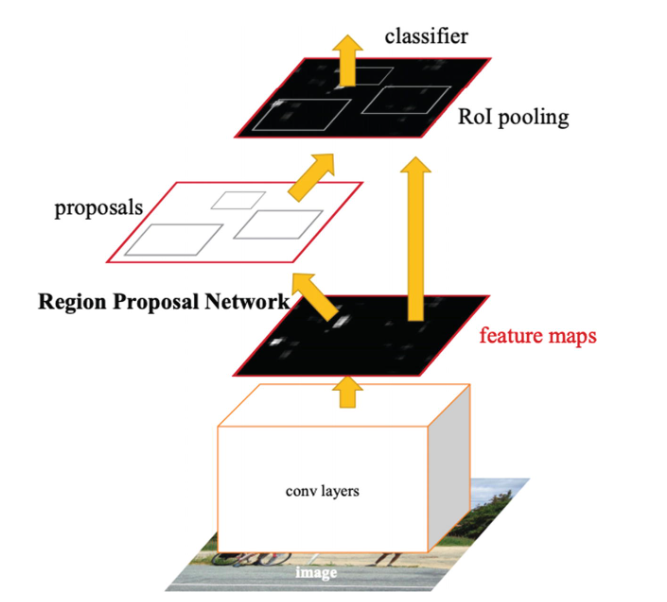
\includegraphics[width=0.7\textwidth]{Faster_RNN.PNG}
    \caption{Architectural Design of Faster R-CNN \cite{ansari2020building}}
    \label{fig:Faster R-CNN}
\end{figure}

\begin{enumerate}
    \item \textbf{Region Proposal Network: } An RPN is a fully convolutional neural network that predicts object bounds and objectness scores simultaneously at each position of the image.
    An RPN is a deep CNN that takes an image input and generates the output as a set of rectangular object proposals. Each rectangular proposal has an “objectness” score.
    
    \begin{figure}[H]
        \centering
        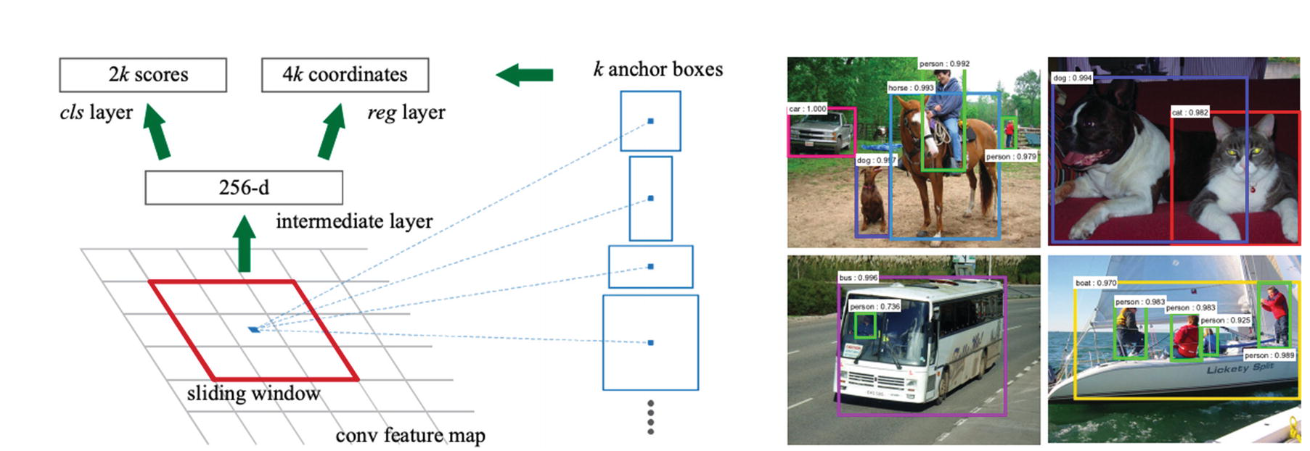
\includegraphics[width=1\textwidth]{RPN.PNG}
        \caption{Region Proposal Networks (RPN) [image source: \cite{chen2018enhanced}}
        \label{fig:RPN}
    \end{figure}
    RPN has a classifier and a regressor. The concept of anchors has been introduced, which refers to the central point of the sliding window.
    The classifier determines the probability of a proposal having the target object. Regression
    regresses the coordinates of the proposals.
    At each sliding window location, the algorithm predicts multiple region proposals. If the maximum number of proposals at each window location is k, then the total number of bounding box coordinates will be 4k, while the number of object classes will be 2k. One of the classes will indicate the probability of an object being present in the region, and the other will indicate the probability of no object being present. These region boxes at each window are referred to as anchors.\\
    \item \textbf{Fast R-CNN: } The Faster R-CNN consists of two parts, with the second part being the detection network. This part is identical to the Fast R-CNN, which was described earlier. The Fast R-CNN uses input from the RPN to detect objects in images.
\end{enumerate} \cite{ansari2020building}, \cite{salvador2016faster}


\subsubsection{Mask R-CNN}
The Mask R-CNN extends the Faster R-CNN. The Mask R-CNN adds another branch for the object class, bounding box coordinates, and predicting an object mask.
Here is how the Mask R-CNN differs from its predecessor, the Faster R-CNN:
\begin{itemize}
    \item The Faster R-CNN algorithm produces two main results, namely: a predicted class label and the coordinates of the bounding box for the object of interest in an image.
    \item The Mask R-CNN has three outputs: a class label, bounding box coordinates, and an object mask.
\end{itemize}
The Mask R-CNN algorithm classifies each pixel of an image into a specific category, without distinguishing between individual object instances. To achieve this, it employs a technique known as pixel-to-pixel alignment between the output and input layers of the neural network. The classification of each pixel is then used to determine the masks in the region of interest (ROI).\cite{he2017mask}

\begin{figure}[H]
    \centering
    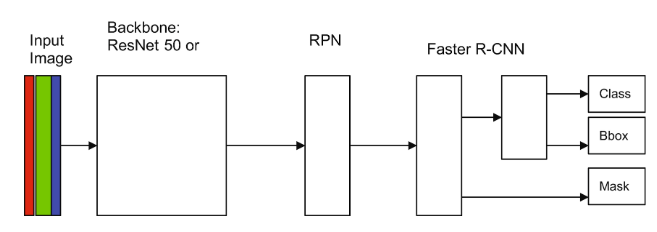
\includegraphics[width=1\textwidth]{MaskR-CNN.PNG}
    \caption{Mask R-CNN network architecture \cite{he2017mask}}
    \label{fig:MaskR-CNN}
\end{figure}
As shown in Figure \ref{fig:MaskR-CNN}, the network consists of three components \textbf{modules—backbone, RPN, and output head}.
\begin{itemize}
    \item \textbf{Backbone} The backbone networks are commonly seen in object detection model architectures. The original paper describes using ResNet-50 and ResNet-101[ \textcolor{red}{\href{https://arxiv.org/pdf/1612.03144.pdf}{Ref1}} ]
    The backbone’s main role is feature extraction.
    In addition to ResNet, a feature pyramid network (FPN) is also utilized to extract the feature details of the image.
    \begin{figure}[H]
        \centering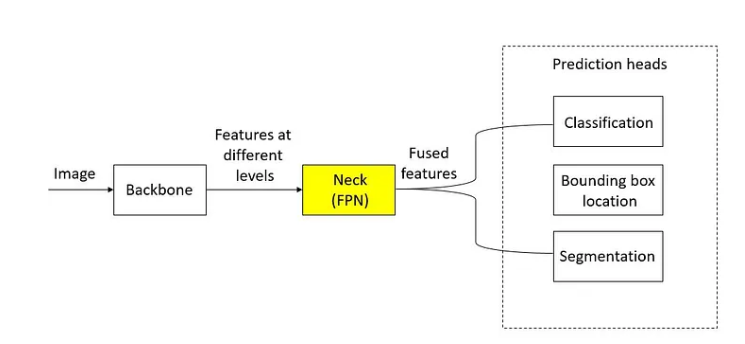
\includegraphics[width=1\textwidth]{BackBone_FPN.PNG}
        \caption{BackBone and FPN Tuning architecture \protect\href{https://medium.com/@freshtechyy/fusing-backbone-features-using-feature-pyramid-network-fpn-c652aa6a264b}{[\textcolor{black}{Ref}} ]}\cite{zhu2022improved} 
    \end{figure}
The FPN consists of decreasing-size layers of a CNN, in which case each forward layer has fewer neurons.

        \item \textbf{Feature Pyramid Network (FPN): } is a neck network that combines features of different resolutions obtained from a backbone network, such as ResNet. A CNN-based backbone applies convolution layers to an input image, which results in a set of feature maps with decreasing resolution due to pooling or convolution with a stride different from one.\\
        The FPN consists of a bottom-up and top-down pathway. In the bottom-up pathway, a backbone network, such as ResNet, extracts features with diminishing spatial resolution.
        As the levels of resolution decrease, the semantic meaning of the feature maps increases, as indicated by the blue thickness of the box boundaries.\\
        The feature maps are fused in the top-down pathway to incorporate rich semantic meaning and precise spatial information, as illustrated in the figure. \ref{fig:FPN_Arch} below. \cite{lin2017feature}
        \begin{figure}[H]
            \centering
            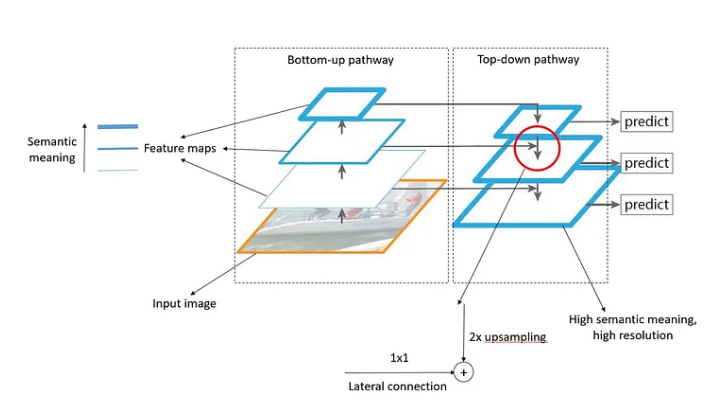
\includegraphics[width=0.7\textwidth]{FPN_Top_bott.PNG}
            \caption{Feature Pyramid Network (FPN) \cite{lin2017feature}}
            \label{fig:FPN_Arch}
        \end{figure}
         \item \textbf{Output Head: } The last module consists of the Faster R-CNN with an additional output branch. \cite{he2017mask}
\end{itemize}
   
\subsection{One stage detector: } 
They can process images in real-time and are suitable for applications where low latency is crucial, such as real-time object detection in video streams or robotics.

\subsubsection{Single-Shot Multibox Detection: }

SSD is primarily designed to solve object detection problems in real-time. An R-CNN and its variants are detectors that work in two stages. They have two specialized networks: one creates the region proposals to predict bounding boxes, and the other predicts the object classes. These detectors are relatively accurate but have a high computational cost. As a result, an R-CNN is not ideal for detecting objects in real-time streaming videos.
A single-shot object detector predicts object classes and bounding boxes in one pass or single forward-pass\cite{liu2016ssd} 
\begin{itemize}
    \item \textbf{SSD Network Architecture: } The SSD approach is a method that uses a feed-forward convolutional network to generate a set of fixed-size bounding boxes and scores, which helps detect the presence of object class instances in those boxes. A non-maximum suppression step is performed in the final stage to obtain the ultimate detections. \\
    \begin{itemize}
        \item \textbfThe {Single Shot MultiBox Detector (SSD)} is a novel object detection framework that adopts grid-based image division instead of the conventional sliding window approach. The SSD approach divides the image into a grid pattern, where each grid cell is responsible for detecting objects within its corresponding region of the image. The objective of object detection is to predict the class and location of an object within its region. In case no object is present, the region is considered a background class, and the location is consequently ignored.

        During the training process, SSD requires only an input image and ground truth boxes for each object. In a convolutional manner, a small set of default boxes of different aspect ratios is evaluated at each location in several feature maps with different scales. For instance, 8x8 and 4x4 in (b) and (c). For each default box, SSD predicts the shape offsets and confidences for all object categories (c1, c2, ..., cp). Notably, these default boxes are first matched to the ground truth boxes during training.
        \begin{figure}[H]
            \centering
            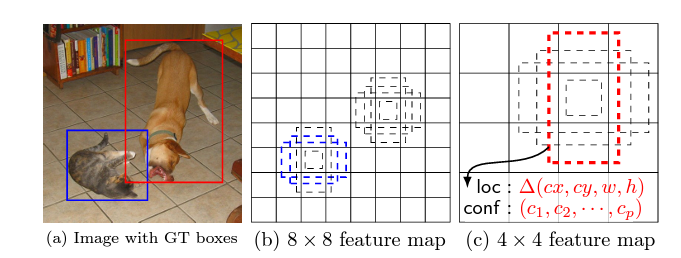
\includegraphics[width=\textwidth]{SSD_GridCell.PNG}
            \caption{SSD:Single Shot Multi-Box Detector \textcolor{red}{\protect\href{https://arxiv.org/pdf/1512.02325.pdf}{image source: \cite{liu2016ssd}}}}
            \label{fig:SSD_grid}
        \end{figure}
        
        \item \textbf{Anchor Boxes:} Object detection is a process by which we aim to identify and locate objects as they appear within an image. This process is different from image classification because there may be multiple objects of the same or different classes present in the image, and object detection seeks to predict all of these objects accurately. In object detection, we use anchor boxes to help locate these objects in the image.
        Object detection models tackle this task by breaking the prediction step into two pieces: 
        \textcolor{red}{\href{https://blog.roboflow.com/what-is-an-anchor-box/}{Ref: Anchor-box}}
        \begin{enumerate}
            \item First, they predict a bounding box through regression and
            \item Second, by predicting a class label through classification.
        \end{enumerate}
        
        \begin{figure}[H]
            \centering
            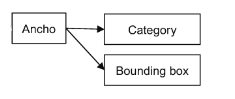
\includegraphics[width=0.2\textwidth]{Anchor.PNG}
            \caption{Anchor}
            \label{fig:anchor}
        \end{figure}
       To detect and locate multiple objects in an image, modern object detection models such as SSD, EfficientDet, and the YOLO models use anchor boxes as a starting point and then make adjustments accordingly. These anchor boxes are predetermined, and each one is responsible for a specific size and shape within a grid cell.

      Anchors are rectangular shapes that are set at each convolution point of the feature map. In SSD, each grid cell can have multiple anchors or prior boxes assigned to it.
            
        
        In Figure \ref{fig: anchor box}, there are five rectangular anchors (shown in red outlines) set at a point (shown in blue).
        \begin{figure}[H]
            \centering
            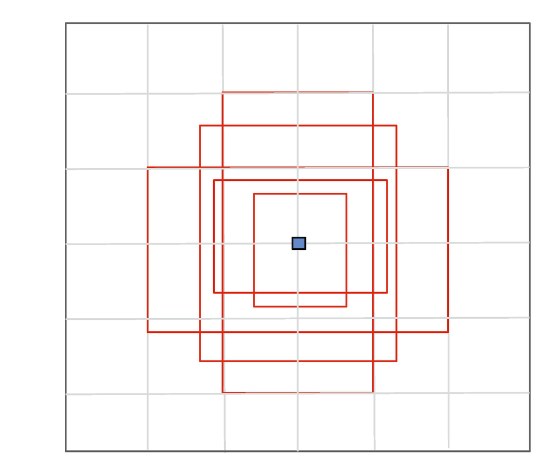
\includegraphics[width=0.5\textwidth]{Anchor_Boxes.PNG}
            \caption{Anchor Boxes}
            \label{fig: anchor box}
        \end{figure}
        In Single Shot Detector (SSD) network, multiple anchor boxes are selected at each location. These anchors serve as detectors, and the different sizes of these detectors enable the detection of objects of varying sizes. Smaller detectors can detect small objects, while larger detectors are capable of detecting larger objects.\\
        \item SSD does not use k-means to determine the anchor boxes, unlike some other object detection algorithms. Instead, it employs a mathematical formula to compute the anchor sizes. As a result, the sizes of SSD's anchor boxes are not dependent on the dataset used. In the SSD paper, these anchor boxes are referred to as "default boxes".\textcolor{red 
        {\href{https://arxiv.org/pdf/1512.02325.pdf}{Ref:Original Paper}}.  \href{https://machinethink.net/blog/object-detection/}{SSD}
        
        It is worth mentioning that in SSD (Single Shot Multibox Detector), anchors are predetermined and set as constants. At each convolution point, a set of fixed "default anchors" is placed. These anchors are associated with a set of default bounding boxes for multiple feature maps at the top of the network. They are laid out in a convolutional manner, tiling the feature map so that the position of each box relative to its corresponding cell remains fixed.
            \end{itemize}
    \item \textbf{Model Architecture: } An SSD neural network consists of two components: \textbf{base network and prediction network.}
    \begin{enumerate}
        \item \textbf{Base network:} The base network is a type of deep convolutional network that is used for feature extraction from input images. It is typically created by removing the fully connected layer of existing networks such as ResNet or VGG. In the case of SSD, the base network is truncated before any classification layer.
        \item \textbf{Detection network:} To the base network, attach some extra convolutional layers that will actually do the prediction of bounding boxes and object classes. 
        \begin{figure}[H]
        \centering
        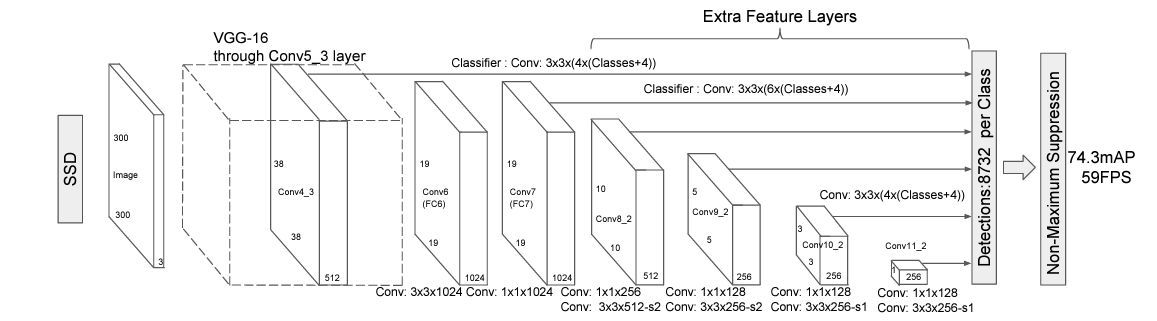
\includegraphics[width=\textwidth]{SSD_ARch.PNG}
        \caption{single shot detection models: SSD \cite{liu2016ssd}}
        \label{fig: single shot detection models: SSD}
        \end{figure}
    The detection network is characterized by the following features: \cite{liu2016ssd}
        \begin{itemize}
            \item TThe layers in the network gradually decrease in size, enabling the detection of objects at multiple scales.
            \item  Each feature layer in the network uses a different convolutional model for predicting detections.
            \item By adding a new feature layer (or using an existing layer from the base network), a fixed set of detection predictions can be generated using a set of convolutional filters
        \end{itemize}
    \end{enumerate}
    \item \textbf{Matching System: } When training, we must choose default boxes that correspond to ground truth detection and train the network accordingly. For each ground truth box, we choose from default boxes that vary in location, aspect ratio, and scale.  The SSD uses IoU (intersection over union) to match the default boxes with the ground truth. This is done by determining the overlap between them. The IoU-based overlap is also known as the Jaccard overlap. If the overlap between the default box and the ground truth is 0.5 or more, it is considered a match. This process of matching is repeated at each layer, which allows the network to learn at scale. Initially, the SSD uses the default boxes as predictions and then tries to regress and come closer to the ground truth bounding boxes. \cite{ansari2020building}, \cite{liu2016ssd}

\end{itemize}

\subsection{Object Detection Evaluation Metrics}
Object detection is a computer vision task where the goal is to identify and locate objects of interest within an image or a video. Several evaluation metrics are commonly used to assess the performance of object detection algorithms. The following are some of the detection metrics:
\subsubsection{Intersection over Union (IoU)}
Intersection over union (IoU), also known as the Jaccard index, is one of the most commonly used evaluation metrics in object detection algorithms. It is used to evaluate the performance of object detection by comparing the ground truth bounding box to the predicted bounding box and IoU.
When it comes to object detection, we create training sets by drawing bounding boxes around objects to label them. These bounding boxes are also known as ground truth in the training set. During the model learning process, the object detection algorithm predicts bounding boxes and then compares them with the ground truth. To determine the accuracy of the predicted bounding box, we use intersection over union (IoU) to evaluate to what extent the predicted bounding box overlaps with the ground truth.\cite{ansari2020building}, \cite{bfortuner_mlglossary}, \cite{liu2016ssd}

\begin{figure}[H]
    \centering
    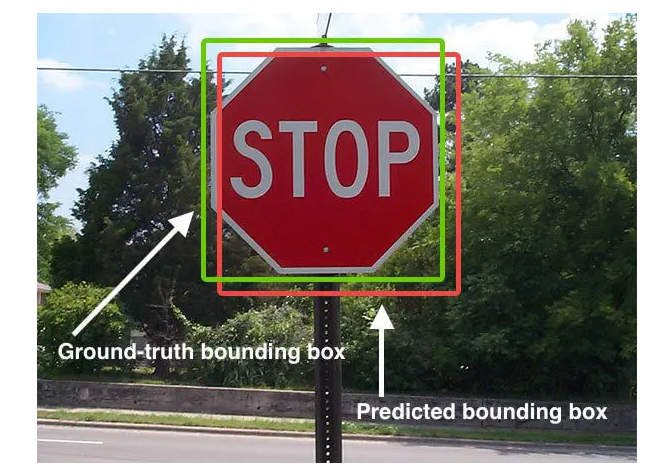
\includegraphics[width=0.6\textwidth]{Intersection_overUnion_(IoU).PNG}
    \caption{The predicted bounding box and Ground-truth bounding box \cite{ansari2020building}}
    \label{fig:PBGTB}
\end{figure}

\textbf{Computing Intersection over Union can therefore be determined as:}\\

\begin{figure}[H]
    \centering
    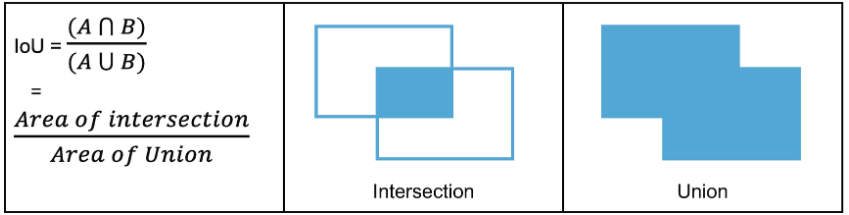
\includegraphics[width=0.6\textwidth]{Intersection_OverUnion.PNG}
    \caption{Intersection OverUnion}
    \label{fig:Intersection_OverUnion}
\end{figure}

\subsubsection{Mean Average Precision (mAP)}
Mean Average Precision (mAP) is a frequently employed metric for evaluating the effectiveness of object identification and segmentation systems. Several object recognition techniques, including Faster R-CNN, MobileNet SSD, and YOLO, utilize mean Average Precision (mAP) as a metric to assess the performance of their models. The mean Average Precision (mAP) is utilized in various benchmark challenges, including Pascal, VOC, COCO, and others. The mean of Average Precision (AP) values are computed by averaging the AP values obtained for recall levels ranging from 0 to 1.\cite{padilla2020survey}, \cite{ansari2020building},  \\
mAP formula is based on the following sub metrics:
\begin{itemize}
    \item Confusion Matrix
    \item Intersection over Union(IoU)
    \item Recall,
    \item Precision
\end{itemize}
\begin{enumerate}
    \item \textbf{Confusion Matrix: }A confusion matrix is a table that is often used to evaluate the performance of a classification algorithm on a set of labeled data for which the true values are known. It provides a summary of the classification results, breaking down the predicted and actual classes into four categories: true positives (TP), true negatives (TN), false positives (FP), and false negatives (FN). \cite{padilla2020survey}, \cite{li2019analysis}
    \begin{itemize}
        \item \textbf{True Positives (TP): } This is when the model accurately predicts a label that matches the ground truth.\\
        \item \textbf{True Negatives (TN): } This is when the model does not predict the label and is not part of the ground truth.\\
        \item  \textbf{False Positives (FP): } This is when the model predicts a label, but it is not a part of the ground truth (Type I Error).\\
        \item \textbf{False Negatives (FN): } Finally, this is when the model does not predict a label, but it is part of the ground truth. (Type II Error).
        \begin{figure}[H]
            \centering
            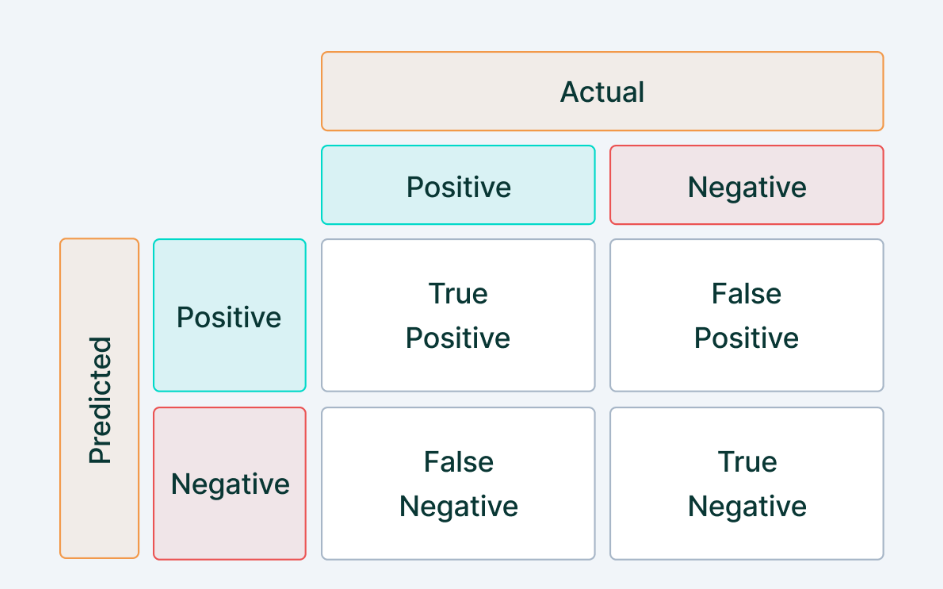
\includegraphics[width=0.7\textwidth]{confusion_matrix.PNG}
            \caption{Confusion matrix table}
            \label{fig:Confusion_Matrix}
        \end{figure}
    \end{itemize}
    \item \textbf{Precision: } Precision measures how well you can find true positives(TP) out of all positive predictions. (TP+FP).
    $$Precision=\frac{TP}{TPTP+FP}$$

    \item \textbf{Recall: } Recall measures how well you can find true positives(TP) out of all predictions(TP+FN).
    $$Recall=\frac{TP}{TPTP+FN}$$
    
  
\end{enumerate}


\subsection{YOLO}
YOLO is one of a real-time object detection algorithm that is aimed and designed to be fast and accurate. It uses a single convolutional neural network to simultaneously predict the bounding boxes along with class probabilities of objects in an image. What sets YOLO apart from other object detection algorithms is that it trains on the full image and is set up to solve regression problems. This means that it does not require a complex processing pipeline, which makes it extremely fast.YOLO is a system that simplifies object detection by treating it as a single regression problem. It predicts bounding box coordinates and class probabilities directly from image pixels. With YOLO, you can detect objects in an image with just one look and get information about what objects are present and where they are located. \cite{redmon2016you}, \cite{ansari2020building}

\subsubsection{Detection Algorithm}
The YOLO design enables end-to-end training and real-time speeds while maintaining high average precision. \\
It divides the image into an SxS grid and for each
grid cell predicts \textbf{B} bounding boxes, confidence for those boxes,
and C-class probabilities. These predictions are encoded as a tensor.
\[
S x S x (B*5 + C)
\]
\\
\begin{figure}[H]
    \centering
    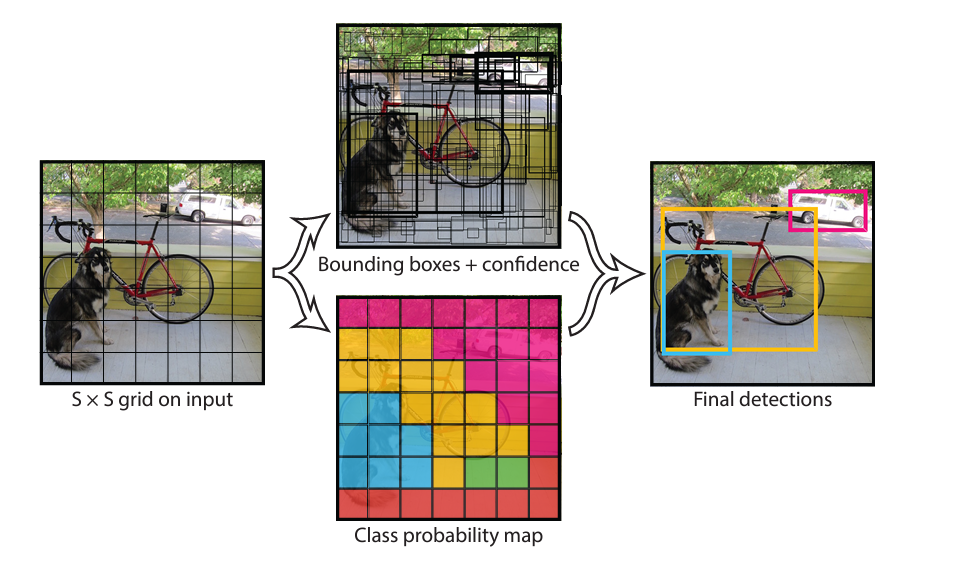
\includegraphics[width=0.8\textwidth]{YOLO_Detection.PNG}
    \caption{YOLO Model \cite{redmon2016you}}
    \label{fig:YoloV1_Model}
\end{figure}

Each bounding box consists of 5 predictions: x, y, w, h,
and confidence. confidence scores reflect how confident the model is.
\[
Confidence =Pr(Object)*IOU_{pred}^{truth}
\]
\subsubsection{YOLO Architectural Design}
The YOLO network architecture is inspired by GoogLeNet and is composed of 24 convolutional layers and 2 fully connected layers for image classification. The YOLO network uses 1x1 reduction layers followed by 3x3 convolutional layers, in contrast to the inception modules used in GoogLeNet. The full network is shown in Figure[\ref{fig:YOLO_arc}].
\begin{figure}[H]
    \centering
    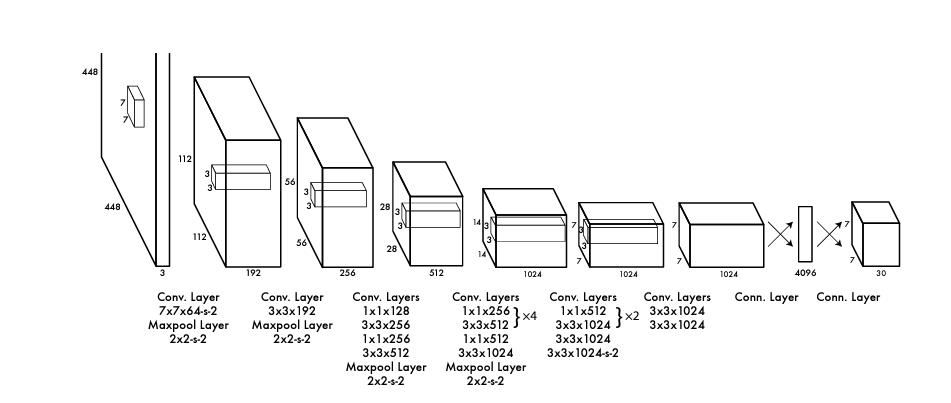
\includegraphics[width=\textwidth]{Yolo_Arch.PNG}
    \caption{YOLO Model (Image source Original paper \cite{redmon2016you})}
    \label{fig:YOLO_arc}
\end{figure}
The convolutional layers were pre-trained on the ImageNet 1000-class competition dataset. Following an average-pooling layer and a fully connected layer, YOLO uses the first 20 convolutional layers from Figure \ref{fig:YOLO_arc} for pretraining. The final layer predicts both class probabilities and bounding box coordinates. A leaky rectified linear activation is used for all layers except the final layer, which uses a linear activation function.
 \[
 \phi(x)=\begin{cases}
           x, & \text{if } x>0 \\
          0.1x, & \text{otherwise}
      \end{cases}
\]

\subsubsection{Limitations of YOLO}
\begin{itemize}
    \item It struggles with small objects that come in groups, such as flocks of birds.
    \item It can predict only one class of objects within a cell grid.
    \item It does not predict well if the object has an unusual aspect ratio that was not seen in the training set.
    \item The accuracy of YOLO is lower than that of Faster R-CNN and some of the state-of-the-art algorithms.
\end{itemize}

\subsection{Transfer Learning and Pre-trained Models:}

Transfer learning is a technique in deep learning where a pre-trained model for a particular task is used as a starting point for another model that performs a similar task. This approach provides a faster and easier way to update and retrain a network as compared to training a network from scratch. It is commonly used in various applications, such as object detection, image recognition, and speech recognition. \cite{you2021logme}

Transfer learning is a popular technique because:
\begin{itemize}
    \item Using transfer learning, you can train models with less labeled data by utilizing popular models that have already been trained on large datasets.
    \item  It can reduce training time and computing resources. With transfer learning, the weights are not learned from scratch because the pre-trained model has already learned the weights based on previous learning.
    \item You can take advantage of model architectures developed by the deep learning research community, including popular architectures such as GoogLeNet and ResNet.
\end{itemize}
\begin{figure}[H]
     \centering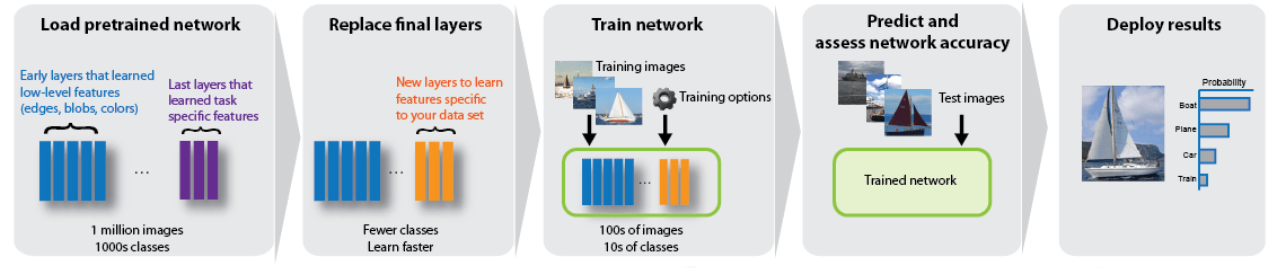
\includegraphics[width=1\linewidth]{Transfer_Learning_Model.PNG}
    \caption{Transfer Learning (Image source: \cite{murugan2021diconet})}
    \label{fig: Transfer Learning}
\end{figure}
\subsubsection{Pre-trained Model}
There are several pre-trained models available for object detection. Below are some of the most popular ones:\\
\begin{itemize}
    \item Alexnet, googlenet(ImageNet), goolgenet(Places365), resnet18, resnet50, resnet101, vgg16, vgg19, inceptionv3, inceptionresnetv2, squeezenet, densenet201, mobilenetv2, shufflenet, xception, nasnetmobile, nasnetlarge. 
\end{itemize}

When selecting a neural network, it's crucial to take into account its accuracy, speed, and size. Usually, there's a trade-off between these factors. To make a well-informed decision, you can refer to the graph below which compares the ImageNet validation accuracy with the time taken for prediction using the neural network. \cite{li2019analysis}
\begin{figure}[H]
    \centering
    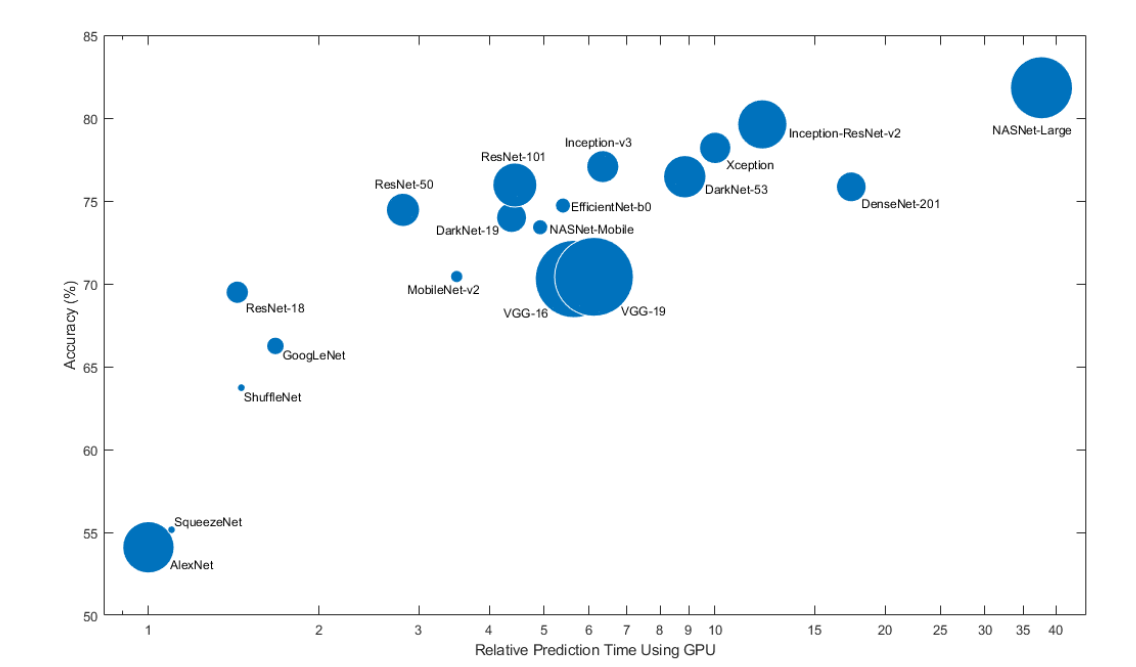
\includegraphics[width=1\textwidth]{Pre-trained_comparision.PNG}
    \caption{Compare Pretrained Neural Networks \cite{YOLo_NAS_Whitepaper_2022}}
    \label{fig: Pretrained Model Comparison}
\end{figure}

